% Options for packages loaded elsewhere
% Options for packages loaded elsewhere
\PassOptionsToPackage{unicode}{hyperref}
\PassOptionsToPackage{hyphens}{url}
\PassOptionsToPackage{dvipsnames,svgnames,x11names}{xcolor}
%
\documentclass[
  spanish,
  us-letterpaper,
  DIV=11,
  numbers=noendperiod]{scrreprt}
\usepackage{xcolor}
\usepackage{amsmath,amssymb}
\setcounter{secnumdepth}{5}
\usepackage{iftex}
\ifPDFTeX
  \usepackage[T1]{fontenc}
  \usepackage[utf8]{inputenc}
  \usepackage{textcomp} % provide euro and other symbols
\else % if luatex or xetex
  \usepackage{unicode-math} % this also loads fontspec
  \defaultfontfeatures{Scale=MatchLowercase}
  \defaultfontfeatures[\rmfamily]{Ligatures=TeX,Scale=1}
\fi
\usepackage{lmodern}
\ifPDFTeX\else
  % xetex/luatex font selection
\fi
% Use upquote if available, for straight quotes in verbatim environments
\IfFileExists{upquote.sty}{\usepackage{upquote}}{}
\IfFileExists{microtype.sty}{% use microtype if available
  \usepackage[]{microtype}
  \UseMicrotypeSet[protrusion]{basicmath} % disable protrusion for tt fonts
}{}
\makeatletter
\@ifundefined{KOMAClassName}{% if non-KOMA class
  \IfFileExists{parskip.sty}{%
    \usepackage{parskip}
  }{% else
    \setlength{\parindent}{0pt}
    \setlength{\parskip}{6pt plus 2pt minus 1pt}}
}{% if KOMA class
  \KOMAoptions{parskip=half}}
\makeatother
% Make \paragraph and \subparagraph free-standing
\makeatletter
\ifx\paragraph\undefined\else
  \let\oldparagraph\paragraph
  \renewcommand{\paragraph}{
    \@ifstar
      \xxxParagraphStar
      \xxxParagraphNoStar
  }
  \newcommand{\xxxParagraphStar}[1]{\oldparagraph*{#1}\mbox{}}
  \newcommand{\xxxParagraphNoStar}[1]{\oldparagraph{#1}\mbox{}}
\fi
\ifx\subparagraph\undefined\else
  \let\oldsubparagraph\subparagraph
  \renewcommand{\subparagraph}{
    \@ifstar
      \xxxSubParagraphStar
      \xxxSubParagraphNoStar
  }
  \newcommand{\xxxSubParagraphStar}[1]{\oldsubparagraph*{#1}\mbox{}}
  \newcommand{\xxxSubParagraphNoStar}[1]{\oldsubparagraph{#1}\mbox{}}
\fi
\makeatother


\usepackage{longtable,booktabs,array}
\usepackage{calc} % for calculating minipage widths
% Correct order of tables after \paragraph or \subparagraph
\usepackage{etoolbox}
\makeatletter
\patchcmd\longtable{\par}{\if@noskipsec\mbox{}\fi\par}{}{}
\makeatother
% Allow footnotes in longtable head/foot
\IfFileExists{footnotehyper.sty}{\usepackage{footnotehyper}}{\usepackage{footnote}}
\makesavenoteenv{longtable}
\usepackage{graphicx}
\makeatletter
\newsavebox\pandoc@box
\newcommand*\pandocbounded[1]{% scales image to fit in text height/width
  \sbox\pandoc@box{#1}%
  \Gscale@div\@tempa{\textheight}{\dimexpr\ht\pandoc@box+\dp\pandoc@box\relax}%
  \Gscale@div\@tempb{\linewidth}{\wd\pandoc@box}%
  \ifdim\@tempb\p@<\@tempa\p@\let\@tempa\@tempb\fi% select the smaller of both
  \ifdim\@tempa\p@<\p@\scalebox{\@tempa}{\usebox\pandoc@box}%
  \else\usebox{\pandoc@box}%
  \fi%
}
% Set default figure placement to htbp
\def\fps@figure{htbp}
\makeatother


% definitions for citeproc citations
\NewDocumentCommand\citeproctext{}{}
\NewDocumentCommand\citeproc{mm}{%
  \begingroup\def\citeproctext{#2}\cite{#1}\endgroup}
\makeatletter
 % allow citations to break across lines
 \let\@cite@ofmt\@firstofone
 % avoid brackets around text for \cite:
 \def\@biblabel#1{}
 \def\@cite#1#2{{#1\if@tempswa , #2\fi}}
\makeatother
\newlength{\cslhangindent}
\setlength{\cslhangindent}{1.5em}
\newlength{\csllabelwidth}
\setlength{\csllabelwidth}{3em}
\newenvironment{CSLReferences}[2] % #1 hanging-indent, #2 entry-spacing
 {\begin{list}{}{%
  \setlength{\itemindent}{0pt}
  \setlength{\leftmargin}{0pt}
  \setlength{\parsep}{0pt}
  % turn on hanging indent if param 1 is 1
  \ifodd #1
   \setlength{\leftmargin}{\cslhangindent}
   \setlength{\itemindent}{-1\cslhangindent}
  \fi
  % set entry spacing
  \setlength{\itemsep}{#2\baselineskip}}}
 {\end{list}}
\usepackage{calc}
\newcommand{\CSLBlock}[1]{\hfill\break\parbox[t]{\linewidth}{\strut\ignorespaces#1\strut}}
\newcommand{\CSLLeftMargin}[1]{\parbox[t]{\csllabelwidth}{\strut#1\strut}}
\newcommand{\CSLRightInline}[1]{\parbox[t]{\linewidth - \csllabelwidth}{\strut#1\strut}}
\newcommand{\CSLIndent}[1]{\hspace{\cslhangindent}#1}

\ifLuaTeX
\usepackage[bidi=basic]{babel}
\else
\usepackage[bidi=default]{babel}
\fi
% get rid of language-specific shorthands (see #6817):
\let\LanguageShortHands\languageshorthands
\def\languageshorthands#1{}


\setlength{\emergencystretch}{3em} % prevent overfull lines

\providecommand{\tightlist}{%
  \setlength{\itemsep}{0pt}\setlength{\parskip}{0pt}}



 


\KOMAoption{captions}{tableheading}
\makeatletter
\@ifpackageloaded{tcolorbox}{}{\usepackage[skins,breakable]{tcolorbox}}
\@ifpackageloaded{fontawesome5}{}{\usepackage{fontawesome5}}
\definecolor{quarto-callout-color}{HTML}{909090}
\definecolor{quarto-callout-note-color}{HTML}{0758E5}
\definecolor{quarto-callout-important-color}{HTML}{CC1914}
\definecolor{quarto-callout-warning-color}{HTML}{EB9113}
\definecolor{quarto-callout-tip-color}{HTML}{00A047}
\definecolor{quarto-callout-caution-color}{HTML}{FC5300}
\definecolor{quarto-callout-color-frame}{HTML}{acacac}
\definecolor{quarto-callout-note-color-frame}{HTML}{4582ec}
\definecolor{quarto-callout-important-color-frame}{HTML}{d9534f}
\definecolor{quarto-callout-warning-color-frame}{HTML}{f0ad4e}
\definecolor{quarto-callout-tip-color-frame}{HTML}{02b875}
\definecolor{quarto-callout-caution-color-frame}{HTML}{fd7e14}
\makeatother
\makeatletter
\@ifpackageloaded{bookmark}{}{\usepackage{bookmark}}
\makeatother
\makeatletter
\@ifpackageloaded{caption}{}{\usepackage{caption}}
\AtBeginDocument{%
\ifdefined\contentsname
  \renewcommand*\contentsname{Tabla de contenidos}
\else
  \newcommand\contentsname{Tabla de contenidos}
\fi
\ifdefined\listfigurename
  \renewcommand*\listfigurename{Listado de Figuras}
\else
  \newcommand\listfigurename{Listado de Figuras}
\fi
\ifdefined\listtablename
  \renewcommand*\listtablename{Listado de Tablas}
\else
  \newcommand\listtablename{Listado de Tablas}
\fi
\ifdefined\figurename
  \renewcommand*\figurename{Figura}
\else
  \newcommand\figurename{Figura}
\fi
\ifdefined\tablename
  \renewcommand*\tablename{Tabla}
\else
  \newcommand\tablename{Tabla}
\fi
}
\@ifpackageloaded{float}{}{\usepackage{float}}
\floatstyle{ruled}
\@ifundefined{c@chapter}{\newfloat{codelisting}{h}{lop}}{\newfloat{codelisting}{h}{lop}[chapter]}
\floatname{codelisting}{Listado}
\newcommand*\listoflistings{\listof{codelisting}{Listado de Listados}}
\makeatother
\makeatletter
\makeatother
\makeatletter
\@ifpackageloaded{caption}{}{\usepackage{caption}}
\@ifpackageloaded{subcaption}{}{\usepackage{subcaption}}
\makeatother
\usepackage{bookmark}
\IfFileExists{xurl.sty}{\usepackage{xurl}}{} % add URL line breaks if available
\urlstyle{same}
\hypersetup{
  pdftitle={Aplicación de Modelos Ocultos de Markov (HMM) al reconocimiento del alfabeto latino},
  pdflang={es},
  colorlinks=true,
  linkcolor={blue},
  filecolor={Maroon},
  citecolor={Blue},
  urlcolor={Blue},
  pdfcreator={LaTeX via pandoc}}


\title{Aplicación de Modelos Ocultos de Markov (HMM) al reconocimiento
del alfabeto latino}
\author{}
\date{}
\begin{document}
\maketitle

\renewcommand*\contentsname{Tabla de contenidos}
{
\hypersetup{linkcolor=}
\setcounter{tocdepth}{2}
\tableofcontents
}

\bookmarksetup{startatroot}

\chapter{Reconocimiento de
Caracteres}\label{reconocimiento-de-caracteres}

\bookmarksetup{startatroot}

\chapter{Espacio Probabilístico y Procesos Estocásticos
Subyacentes}\label{espacio-probabiluxedstico-y-procesos-estocuxe1sticos-subyacentes}

Para establecer formalmente una Cadena de Markov a Tiempo Continuo
(CTMC), es necesario partir de los axiomas fundamentales de la teoría de
la medida, para más detalle consultar el libro de Rudin (1987).

Para esto, se asumirá que el lector tiene conocimientos previos sobre
teoría de la medida como lo son las \(\sigma\)-álgebras, espacio
muestral y medida de probabilidad, entre otros.

\begin{tcolorbox}[enhanced jigsaw, colbacktitle=quarto-callout-note-color!10!white, toptitle=1mm, breakable, colframe=quarto-callout-note-color-frame, left=2mm, toprule=.15mm, opacitybacktitle=0.6, opacityback=0, rightrule=.15mm, bottomtitle=1mm, titlerule=0mm, coltitle=black, colback=white, title=\textcolor{quarto-callout-note-color}{\faInfo}\hspace{0.5em}{Definición (Espacio de Probabilidad Filtrado)}, arc=.35mm, bottomrule=.15mm, leftrule=.75mm]

Sea \((\Omega, \mathcal{F}, \mathbb{P})\) un espacio de probabilidad,
donde \(\Omega\) es el espacio muestral, \(\mathcal{F}\) es una
\(\sigma\)-álgebra sobre \(\Omega\), y \(\mathbb{P}\) es una medida de
probabilidad. Sea \(\mathbb{F} = \{\mathcal{F}_t\}_{t \ge 0}\) una
filtración, es decir, una familia no decreciente de
sub-\(\sigma\)-álgebras de \(\mathcal{F}\) tal que
\(\mathcal{F}_s \subseteq \mathcal{F}_t \subseteq \mathcal{F}\) para
todo \(0 \le s < t\). El conjunto
\((\Omega, \mathcal{F}, \mathbb{F}, \mathbb{P})\) se denomina espacio de
probabilidad filtrado.

\end{tcolorbox}

\begin{tcolorbox}[enhanced jigsaw, colbacktitle=quarto-callout-note-color!10!white, toptitle=1mm, breakable, colframe=quarto-callout-note-color-frame, left=2mm, toprule=.15mm, opacitybacktitle=0.6, opacityback=0, rightrule=.15mm, bottomtitle=1mm, titlerule=0mm, coltitle=black, colback=white, title=\textcolor{quarto-callout-note-color}{\faInfo}\hspace{0.5em}{Definición (Espacio de Estados Discreto)}, arc=.35mm, bottomrule=.15mm, leftrule=.75mm]

Definimos el espacio de estados \(S\) como un conjunto discreto y finito
(o numerable).

La topología en \(S\) es discreta y su \(\sigma\)-álgebra asociada es el
conjunto potencia \(\mathcal{P}(S)\).

\end{tcolorbox}

En el contexto de nuestro proyecto, \(S\) representa el conjunto de
posibles colores o intensidades de un pixel (por ejemplo, el espacio RGB
donde \(|S| = 256^3\), o una escala de grises finita).

\begin{tcolorbox}[enhanced jigsaw, colbacktitle=quarto-callout-note-color!10!white, toptitle=1mm, breakable, colframe=quarto-callout-note-color-frame, left=2mm, toprule=.15mm, opacitybacktitle=0.6, opacityback=0, rightrule=.15mm, bottomtitle=1mm, titlerule=0mm, coltitle=black, colback=white, title=\textcolor{quarto-callout-note-color}{\faInfo}\hspace{0.5em}{Definición (Proceso Estocástico a Tiempo Continuo)}, arc=.35mm, bottomrule=.15mm, leftrule=.75mm]

Un proceso estocástico en tiempo continuo con espacio de estados
discreto \(S\) es una familia de variables aleatorias

\[
X = \{X(t) : t \in \mathbb{R}_{\ge 0}\},
\]

donde cada \(X(t): \Omega \to S\) es una función medible respecto a
\(\mathcal{F}_t\).

\end{tcolorbox}

Interpretamos \(X(t)\) como el ``color verdadero'' del pixel en el
instante (o parámetro continuo) \(t\).

\bookmarksetup{startatroot}

\chapter{Cadenas de Markov a Tiempo Continuo
(CTMC)}\label{cadenas-de-markov-a-tiempo-continuo-ctmc}

La transición del concepto general de proceso estocástico al de proceso
de Markov requiere la propiedad de amnesia (pérdida de memoria).

\begin{tcolorbox}[enhanced jigsaw, colbacktitle=quarto-callout-note-color!10!white, toptitle=1mm, breakable, colframe=quarto-callout-note-color-frame, left=2mm, toprule=.15mm, opacitybacktitle=0.6, opacityback=0, rightrule=.15mm, bottomtitle=1mm, titlerule=0mm, coltitle=black, colback=white, title=\textcolor{quarto-callout-note-color}{\faInfo}\hspace{0.5em}{Definición (Propiedad de Markov)}, arc=.35mm, bottomrule=.15mm, leftrule=.75mm]

El proceso adaptado \(X = \{X(t)\}_{t \ge 0}\) es una Cadena de Markov a
Tiempo Continuo si satisface la condición de Markov relativa a la
filtración \(\mathbb{F}\): para cualquier conjunto discreto de tiempos

\[
0 \le t_1 < t_2 < \dots < t_n < t
\]

y cualquier secuencia de estados

\[
i_1, i_2, \dots, i_n, i, j \in S,
\]

se cumple que

\[
\mathbb{P}(X(t) = j \mid X(t_1) = i_1, \dots, X(t_n) = i, X(s) = i)
=
\mathbb{P}(X(t) = j \mid X(s) = i).
\]

De manera equivalente y más elegante mediante la esperanza condicional:

\[
\mathbb{P}(X(t) = j \mid \mathcal{F}_s)
=
\mathbb{P}(X(t) = j \mid X(s))
\quad
\text{c.s. (casi seguramente)}
\]

para todo \(0 \le s \le t\).

\end{tcolorbox}

\begin{tcolorbox}[enhanced jigsaw, colbacktitle=quarto-callout-note-color!10!white, toptitle=1mm, breakable, colframe=quarto-callout-note-color-frame, left=2mm, toprule=.15mm, opacitybacktitle=0.6, opacityback=0, rightrule=.15mm, bottomtitle=1mm, titlerule=0mm, coltitle=black, colback=white, title=\textcolor{quarto-callout-note-color}{\faInfo}\hspace{0.5em}{Definición (Probabilidades de Transición y Homogeneidad)}, arc=.35mm, bottomrule=.15mm, leftrule=.75mm]

Definimos la probabilidad de transición del estado \(i\) al estado \(j\)
en el intervalo \([s,t]\) como

\[
p_{ij}(s,t)
=
\mathbb{P}(X(t)=j \mid X(s)=i).
\]

Se dice que la CTMC es \textbf{homogénea en el tiempo} si
\(p_{ij}(s,t)\) depende únicamente de la longitud del intervalo temporal

\[
\tau=t-s.
\]

En tal caso, denotamos la probabilidad de transición como

\[
p_{ij}(\tau)
=
\mathbb{P}(X(s+\tau)=j \mid X(s)=i).
\]

Sean estas probabilidades las entradas de una matriz estocástica

\[
P(\tau)
=
[p_{ij}(\tau)]_{i,j\in S}.
\]

\end{tcolorbox}

\begin{tcolorbox}[enhanced jigsaw, colbacktitle=quarto-callout-important-color!10!white, toptitle=1mm, breakable, colframe=quarto-callout-important-color-frame, left=2mm, toprule=.15mm, opacitybacktitle=0.6, opacityback=0, rightrule=.15mm, bottomtitle=1mm, titlerule=0mm, coltitle=black, colback=white, title=\textcolor{quarto-callout-important-color}{\faExclamation}\hspace{0.5em}{Propiedad (Ecuaciones de Chapman-Kolmogorov)}, arc=.35mm, bottomrule=.15mm, leftrule=.75mm]

Para cualquier \(s,t \ge 0\), la familia de matrices de transición
\(\{P(t)\}_{t\ge0}\) forma un semigrupo de operadores estocásticos,
satisfaciendo

\[
P(t+s)=P(t)P(s)
\]

lo que equivale a

\[
p_{ij}(t+s)
=
\sum_{k\in S}
p_{ik}(t)p_{kj}(s).
\]

\end{tcolorbox}

\begin{figure}

\centering{

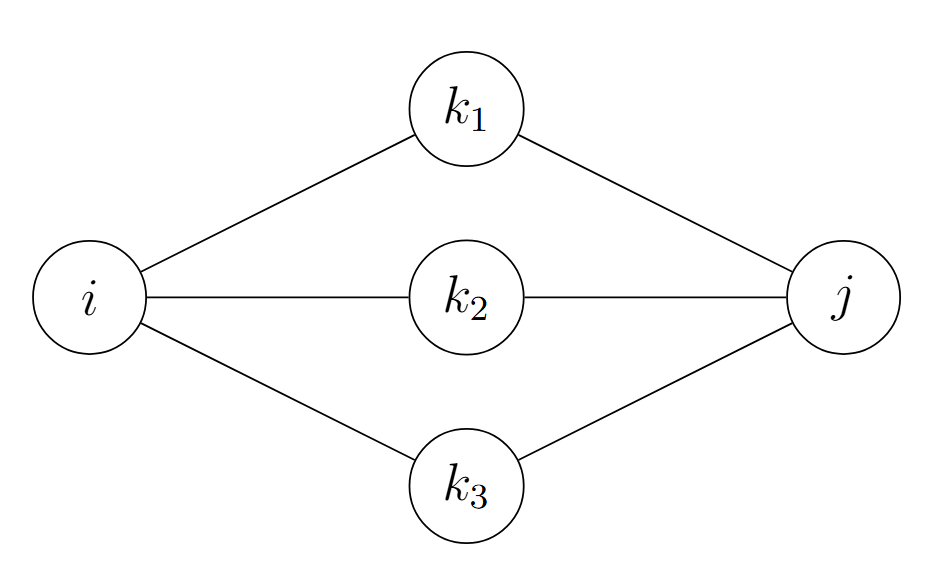
\includegraphics[width=7.29167in,height=\textheight,keepaspectratio]{chapman-k.png}

}

\caption{\label{fig-chapman}La probabilidad de transición
\(p\_{ij}(t+s)\) se obtiene sumando las contribuciones de todos los
posibles estados intermedios \(k\).}

\end{figure}%

\bookmarksetup{startatroot}

\chapter{Dinámica Infinitesimal y Generador de la
Cadena}\label{dinuxe1mica-infinitesimal-y-generador-de-la-cadena}

La evolución continua del color del pixel requiere una descripción
mediante probabilidades de transición, lo cual nos lleva a la
representación matricial de la derivada de \(P(t)\).

\begin{tcolorbox}[enhanced jigsaw, colbacktitle=quarto-callout-note-color!10!white, toptitle=1mm, breakable, colframe=quarto-callout-note-color-frame, left=2mm, toprule=.15mm, opacitybacktitle=0.6, opacityback=0, rightrule=.15mm, bottomtitle=1mm, titlerule=0mm, coltitle=black, colback=white, title=\textcolor{quarto-callout-note-color}{\faInfo}\hspace{0.5em}{Definición (Matriz Generadora Infinitesimal)}, arc=.35mm, bottomrule=.15mm, leftrule=.75mm]

Asumiendo que \(p_{ij}(t)\) es diferenciable por la derecha en \(t=0\),
definimos la tasa de transición \(q_{ij}\) del estado \(i\) al estado
\(j\) (donde \(i \neq j\)) como:

\[
q_{ij}
=
\lim_{h \to 0^+}
\frac{p_{ij}(h)}{h}
\ge 0.
\]

Y para el caso \(i=j\), definimos la probabilidad de salida del estado
\(i\) como \(v_i=-q_{ii}\), dada por

\[
q_{ii}
=
\lim_{h\to0^+}
\frac{p_{ii}(h)-1}{h}
=
-\sum_{j\neq i} q_{ij}
\le 0.
\]

La matriz

\[
Q=[q_{ij}]_{i,j\in S}
\]

se denomina matriz generadora (o matriz \(Q\)) de la cadena. Sus filas
suman cero:

\[
\sum_{j\in S} q_{ij}=0.
\]

\end{tcolorbox}

\begin{tcolorbox}[enhanced jigsaw, colbacktitle=quarto-callout-important-color!10!white, toptitle=1mm, breakable, colframe=quarto-callout-important-color-frame, left=2mm, toprule=.15mm, opacitybacktitle=0.6, opacityback=0, rightrule=.15mm, bottomtitle=1mm, titlerule=0mm, coltitle=black, colback=white, title=\textcolor{quarto-callout-important-color}{\faExclamation}\hspace{0.5em}{Propiedad (Ecuaciones Diferenciales de Kolmogorov)}, arc=.35mm, bottomrule=.15mm, leftrule=.75mm]

Bajo condiciones de regularidad (que se cumplen trivialmente si el
espacio de estados del color \(S\) es finito), la matriz de transición
\(P(t)\) es la solución única a las ecuaciones diferenciales matriciales
de Kolmogorov Hacia Adelante (Forward) y Hacia Atrás (Backward) Norris
(1998) :

\begin{itemize}
\tightlist
\item
  \textbf{Forward:}
\end{itemize}

\[
\frac{d}{dt}P(t)=P(t)Q
\]

\begin{itemize}
\tightlist
\item
  \textbf{Backward:}
\end{itemize}

\[
\frac{d}{dt}P(t)=QP(t)
\]

Cuya solución formal, bajo la condición inicial \(P(0)=I\) (matriz
identidad), es la matriz exponencial

\[
P(t)
=
e^{Qt}
=
\sum_{n=0}^{\infty}
\frac{(Qt)^n}{n!}.
\]

\end{tcolorbox}

\bookmarksetup{startatroot}

\chapter{Utilidad hacia Cadenas de Márkov Ocultas
(HMM)}\label{utilidad-hacia-cadenas-de-muxe1rkov-ocultas-hmm}

La fundamentación teórica precedente modela la dinámica subyacente
determinista de la matriz de transición y la evolución estocástica de
las trayectorias del sistema. Para extender esta arquitectura a un
Modelo Oculto de Márkov (HMM) en el contexto de la inferencia y análisis
de píxeles en imágenes que contienen letras del alfabeto latino, se
formaliza la siguiente estructura bivariada:

\begin{tcolorbox}[enhanced jigsaw, colbacktitle=quarto-callout-note-color!10!white, toptitle=1mm, breakable, colframe=quarto-callout-note-color-frame, left=2mm, toprule=.15mm, opacitybacktitle=0.6, opacityback=0, rightrule=.15mm, bottomtitle=1mm, titlerule=0mm, coltitle=black, colback=white, title=\textcolor{quarto-callout-note-color}{\faInfo}\hspace{0.5em}{Definición (Proceso Latente e Inobservable)}, arc=.35mm, bottomrule=.15mm, leftrule=.75mm]

El proceso de Markov a tiempo continuo

\[
X = \{X(t)\}_{t \ge 0}
\]

sobre el espacio de estados \(S\), caracterizado por su matriz
generadora infinitesimal \(Q\), constituye el \emph{proceso latente}.
Las alteraciones estocásticas inducidas por \(Q\) a lo largo del
parámetro \(t\) (representando una métrica de degradación física o
divergencia espacial) rigen las transiciones hacia estados degradados,
manteniéndose inaccesibles a la medición directa.

\end{tcolorbox}

La variable \(X(t)\) describe el estado ideal o ``verdadero'' del pixel.

\begin{tcolorbox}[enhanced jigsaw, colbacktitle=quarto-callout-note-color!10!white, toptitle=1mm, breakable, colframe=quarto-callout-note-color-frame, left=2mm, toprule=.15mm, opacitybacktitle=0.6, opacityback=0, rightrule=.15mm, bottomtitle=1mm, titlerule=0mm, coltitle=black, colback=white, title=\textcolor{quarto-callout-note-color}{\faInfo}\hspace{0.5em}{Definición (Proceso de Observación Empírica)}, arc=.35mm, bottomrule=.15mm, leftrule=.75mm]

Sea

\[
(O,\mathcal{P}(O))
\]

el espacio medible de las posibles mediciones obtenidas por
instrumentos.

Se postula un \emph{proceso de observación} acoplado

\[
Y=\{Y(t)\}_{t\ge0},
\]

compuesto por variables aleatorias

\[
Y(t):\Omega\to O
\]

que representan la lectura empírica o ruidosa en el parámetro \(t\).

\end{tcolorbox}

En este caso \(O\) denota el conjunto finito de colores o intensidades
registrables por un sensor óptico y \(Y\) es la lectura ruidosa del
pixel en el tiempo \(t\).

\begin{tcolorbox}[enhanced jigsaw, colbacktitle=quarto-callout-note-color!10!white, toptitle=1mm, breakable, colframe=quarto-callout-note-color-frame, left=2mm, toprule=.15mm, opacitybacktitle=0.6, opacityback=0, rightrule=.15mm, bottomtitle=1mm, titlerule=0mm, coltitle=black, colback=white, title=\textcolor{quarto-callout-note-color}{\faInfo}\hspace{0.5em}{Definición (Matriz de Emisión e Independencia Condicional)}, arc=.35mm, bottomrule=.15mm, leftrule=.75mm]

La dependencia estocástica entre ambos procesos queda unívocamente
determinada por la condición de independencia local.

Para cualquier instante \(t\ge0\), la observación \(Y(t)\) es
condicionalmente independiente de toda la historia previa del sistema
dado el estado concurrente \(X(t)\).

Formalmente, para cualquier \(y\in O\) y \(x\in S\):

\[
\mathbb{P}(Y(t)=y \mid \mathcal{F}_t^X,\mathcal{F}_{t^-}^Y)
=
\mathbb{P}(Y(t)=y \mid X(t)=x)
\quad
\text{c.s.}
\]

donde \(\mathcal{F}_t^X\) y \(\mathcal{F}_{t^-}^Y\) denotan las
filtraciones del historial latente y observable, respectivamente.

Estas probabilidades definen las entradas de la matriz de emisión
estocástica

\[
E=[e_{xy}],
\]

donde

\[
e_{xy}
=
\mathbb{P}(Y(t)=y \mid X(t)=x).
\]

\end{tcolorbox}

\bookmarksetup{startatroot}

\chapter{Inferencia y Filtrado en el Modelo
Oculto}\label{inferencia-y-filtrado-en-el-modelo-oculto}

Una vez establecida la dinámica del sistema, es necesario desarrollar la
maquinaria analítica para inferir el estado latente del pixel a partir
de las observaciones empíricas.

Supongamos que disponemos de una secuencia de observaciones

\[
Y=(y_1,y_2,\dots,y_K)
\]

en instantes discretos de tiempo (o espacio)

\[
0 \le t_1 < t_2 < \dots < t_K \le T.
\]

\begin{tcolorbox}[enhanced jigsaw, colbacktitle=quarto-callout-note-color!10!white, toptitle=1mm, breakable, colframe=quarto-callout-note-color-frame, left=2mm, toprule=.15mm, opacitybacktitle=0.6, opacityback=0, rightrule=.15mm, bottomtitle=1mm, titlerule=0mm, coltitle=black, colback=white, title=\textcolor{quarto-callout-note-color}{\faInfo}\hspace{0.5em}{Definición (Filtro Hacia Adelante (Forward) y Verosimilitud)}, arc=.35mm, bottomrule=.15mm, leftrule=.75mm]

Definimos la variable de avance \(\alpha_k(i)\) como la probabilidad
conjunta de observar la secuencia parcial hasta el \(k\)-ésimo instante
y que el estado oculto en dicho instante sea \(i\in S\):

\[
\alpha_k(i)
=
\mathbb{P}
\bigl(
Y(t_1)=y_1,\dots,Y(t_k)=y_k,
X(t_k)=i
\bigr).
\]

Esta cantidad se calcula recursivamente mediante la ecuación de
Chapman-Kolmogorov y la matriz de emisión:

\[
\alpha_k(j)
=
\left(
\sum_{i\in S}
\alpha_{k-1}(i)\,
p_{ij}(\Delta t_k)
\right)
\mathbb{P}
\bigl(
Y(t_k)=y_k
\mid
X(t_k)=j
\bigr)
\]

donde

\[
\Delta t_k=t_k-t_{k-1}
\]

y

\[
p_{ij}(\Delta t_k)
\]

es la entrada correspondiente de la matriz de transición

\[
P(\Delta t_k)
=
e^{Q\Delta t_k}.
\]

La verosimilitud total de la secuencia de observaciones es simplemente

\[
\mathbb{P}(Y)
=
\sum_{i\in S}
\alpha_K(i).
\]

\end{tcolorbox}

\begin{tcolorbox}[enhanced jigsaw, colbacktitle=quarto-callout-note-color!10!white, toptitle=1mm, breakable, colframe=quarto-callout-note-color-frame, left=2mm, toprule=.15mm, opacitybacktitle=0.6, opacityback=0, rightrule=.15mm, bottomtitle=1mm, titlerule=0mm, coltitle=black, colback=white, title=\textcolor{quarto-callout-note-color}{\faInfo}\hspace{0.5em}{Definición (Decodificación Óptima Global)}, arc=.35mm, bottomrule=.15mm, leftrule=.75mm]

Para reconstruir la trayectoria más probable, buscamos la secuencia de
estados latentes

\[
\hat{X}
=
(\hat{x}_1,\dots,\hat{x}_K)
\]

que maximice la probabilidad condicional conjunta

\[
\hat{X}
=
\arg\max_{x_1,\dots,x_K}
\mathbb{P}
\Bigl(
X(t_1)=x_1,\dots,X(t_K)=x_K
\mid
Y(t_1)=y_1,\dots,Y(t_K)=y_K
\Bigr).
\]

La solución sistemática a este problema de programación dinámica
espacial/temporal se obtiene mediante la adaptación del Algoritmo de
Viterbi para cadenas a tiempo continuo, evaluando las transiciones
máximas sobre

\[
P(\Delta t_k).
\]

\end{tcolorbox}

Para los pixeles es la trayectoria más probable de los colores
verdaderos del pixel (el problema de decodificación).

\section{Ejemplo ilustrativo del algoritmo
Forward--Backward}\label{ejemplo-ilustrativo-del-algoritmo-forwardbackward}

Para ilustrar el funcionamiento de los algoritmos Forward y Backward en
el contexto del reconocimiento de imágenes, consideremos un píxel cuyo
color verdadero puede encontrarse en uno de dos estados ocultos:

\[
S=\{B,N\},
\]

donde:

\begin{itemize}
\tightlist
\item
  \(B\): píxel verdaderamente blanco.
\item
  \(N\): píxel verdaderamente negro.
\end{itemize}

Debido al ruido en el proceso de adquisición de la imagen, el color
observado puede diferir del color real.

Supongamos que la dinámica del píxel está descrita por la matriz de
transición

\[
P=
\begin{pmatrix}
0.8 & 0.2\\
0.3 & 0.7
\end{pmatrix},
\]

donde, por ejemplo,

\[
p_{BN}=0.2
\]

representa la probabilidad de que un píxel blanco pase al estado negro
en el siguiente instante.

Asimismo, consideremos la siguiente matriz de emisión:

\[
E=
\begin{pmatrix}
0.9 & 0.1\\
0.2 & 0.8
\end{pmatrix},
\]

cuyas columnas corresponden a las observaciones

\[
(O_B,O_N),
\]

es decir, observar blanco u observar negro. Por ejemplo,

\[
P(O_B \mid B)=0.9,
\qquad
P(O_B \mid N)=0.2.
\]

Finalmente, asumimos una distribución inicial

\[
\pi=(0.6,0.4),
\]

y que la secuencia observada es

\[
Y=(O_B,O_N).
\]

Esto significa que el sensor registra blanco en el primer instante y
negro en el segundo.

\subsection{Cálculo Forward}\label{cuxe1lculo-forward}

La variable Forward se define como

\[
\alpha_k(i)
=
P(y_1,\ldots,y_k,X_k=i).
\]

\subsubsection{Paso 1}\label{paso-1}

Para la primera observación \(O_B\):

\[
\alpha_1(B)
=
P(X_1=B)\,P(O_B\mid B)
=
0.6(0.9)
=
0.54,
\]

\[
\alpha_1(N)
=
P(X_1=N)\,P(O_B\mid N)
=
0.4(0.2)
=
0.08.
\]

\subsubsection{Paso 2}\label{paso-2}

Calculamos primero la probabilidad de alcanzar el estado blanco:

\[
\sum_{i\in S}
\alpha_1(i)p_{iB}
=
0.54(0.8)+0.08(0.3)
=
0.456.
\]

Multiplicando por la probabilidad de emisión correspondiente,

\[
\alpha_2(B)
=
0.456(0.1)
=
0.0456.
\]

Análogamente, para el estado negro:

\[
\sum_{i\in S}
\alpha_1(i)p_{iN}
=
0.54(0.2)+0.08(0.7)
=
0.164,
\]

y por tanto,

\[
\alpha_2(N)
=
0.164(0.8)
=
0.1312.
\]

\subsubsection{Verosimilitud de la secuencia
observada}\label{verosimilitud-de-la-secuencia-observada}

La probabilidad total de observar la secuencia \(Y\) es

\[
P(Y)
=
\alpha_2(B)+\alpha_2(N),
\]

es decir,

\[
P(Y)
=
0.0456+0.1312
=
0.1768.
\]

\subsection{Cálculo Backward}\label{cuxe1lculo-backward}

La variable Backward se define mediante

\[
\beta_k(i)
=
P(y_{k+1},\ldots,y_T\mid X_k=i).
\]

Como la secuencia contiene únicamente dos observaciones,

\[
\beta_2(B)=\beta_2(N)=1.
\]

Retrocediendo un paso:

\[
\beta_1(B)
=
0.8(0.1)(1)
+
0.2(0.8)(1)
=
0.24,
\]

y

\[
\beta_1(N)
=
0.3(0.1)(1)
+
0.7(0.8)(1)
=
0.59.
\]

\subsection{Inferencia del estado
oculto}\label{inferencia-del-estado-oculto}

Una de las principales ventajas del algoritmo Forward--Backward es que
permite calcular la probabilidad posterior de cada estado oculto.

Para el estado blanco en el primer instante,

\[
\gamma_1(B)
=
P(X_1=B\mid Y)
=
\frac{\alpha_1(B)\beta_1(B)}
{P(Y)},
\]

por lo que

\[
\gamma_1(B)
=
\frac{0.54(0.24)}
{0.1768}
=
0.733.
\]

De forma análoga,

\[
\gamma_1(N)
=
\frac{\alpha_1(N)\beta_1(N)}
{P(Y)}
=
\frac{0.08(0.59)}
{0.1768}
=
0.267.
\]

En consecuencia,

\[
P(X_1=B\mid Y)\approx 73.3\%,
\]

mientras que

\[
P(X_1=N\mid Y)\approx 26.7\%.
\]

\textbf{Interpretación}

A pesar de que el sensor observa un píxel blanco en el primer instante y
negro en el segundo, el algoritmo Forward--Backward determina que existe
aproximadamente un \(73\%\) de probabilidad de que el color verdadero
inicial haya sido blanco. Este resultado muestra cómo un Modelo Oculto
de Markov combina la información proporcionada por las observaciones
ruidosas con la dinámica de transición del sistema para inferir el
estado real subyacente del píxel.

\begin{figure}

\centering{

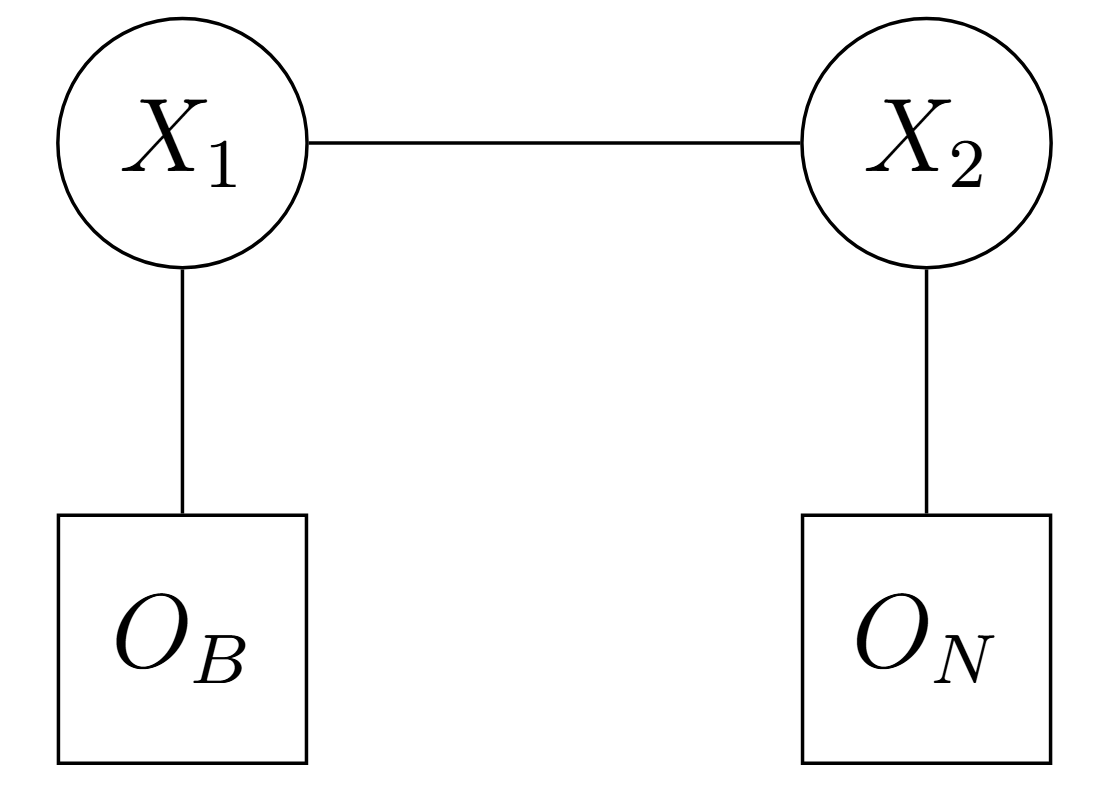
\includegraphics[width=4.6875in,height=\textheight,keepaspectratio]{imagenesHMM/pixelblanconegrodibujo.png}

}

\caption{\label{fig-pixelbn}Modelo Oculto de Markov para un píxel con
dos estados ocultos y dos observaciones.}

\end{figure}%

\bookmarksetup{startatroot}

\chapter{Estimación de Parámetros y Calibración del
Modelo}\label{estimaciuxf3n-de-paruxe1metros-y-calibraciuxf3n-del-modelo}

En la práctica, la matriz generadora infinitesimal \(Q\) (que dicta la
tasa de degradación del color para el caso de estudio) y las
probabilidades de emisión empírica rara vez son conocidas a priori y
deben ser estimadas a partir de un dataset de imágenes (el alfabeto
latino modificado).

\begin{tcolorbox}[enhanced jigsaw, colbacktitle=quarto-callout-important-color!10!white, toptitle=1mm, breakable, colframe=quarto-callout-important-color-frame, left=2mm, toprule=.15mm, opacitybacktitle=0.6, opacityback=0, rightrule=.15mm, bottomtitle=1mm, titlerule=0mm, coltitle=black, colback=white, title=\textcolor{quarto-callout-important-color}{\faExclamation}\hspace{0.5em}{Propiedad (Algoritmo de Expectation-Maximization (Baum-Welch))}, arc=.35mm, bottomrule=.15mm, leftrule=.75mm]

La estimación por máxima verosimilitud del conjunto de parámetros del
modelo

\[
\Theta=\{Q,E\}
\]

dado un conjunto de secuencias observadas se realiza mediante un proceso
iterativo.

\begin{itemize}
\item
  \textbf{Paso E (Expectation):} Se calculan las estadísticas
  suficientes esperadas del sistema latente (tiempo esperado de
  permanencia en cada estado de color y número esperado de transiciones)
  condicionado a las observaciones y a la estimación actual de los
  parámetros \(\Theta^{(m)}\), utilizando las variables recursivas
  Forward y Backward.
\item
  \textbf{Paso M (Maximization):} Se actualizan los parámetros
  \(\Theta^{(m+1)}\) para maximizar la función Q de verosimilitud
  esperada. En particular, la estimación de las probabilidades de
  transición empíricas se formula restringiendo las soluciones para
  garantizar que las filas de \(Q^{(m+1)}\) sigan sumando cero y
  \(q_{ij}\ge0\) para \(i\neq j\).
\end{itemize}

\end{tcolorbox}

\begin{figure}

\centering{

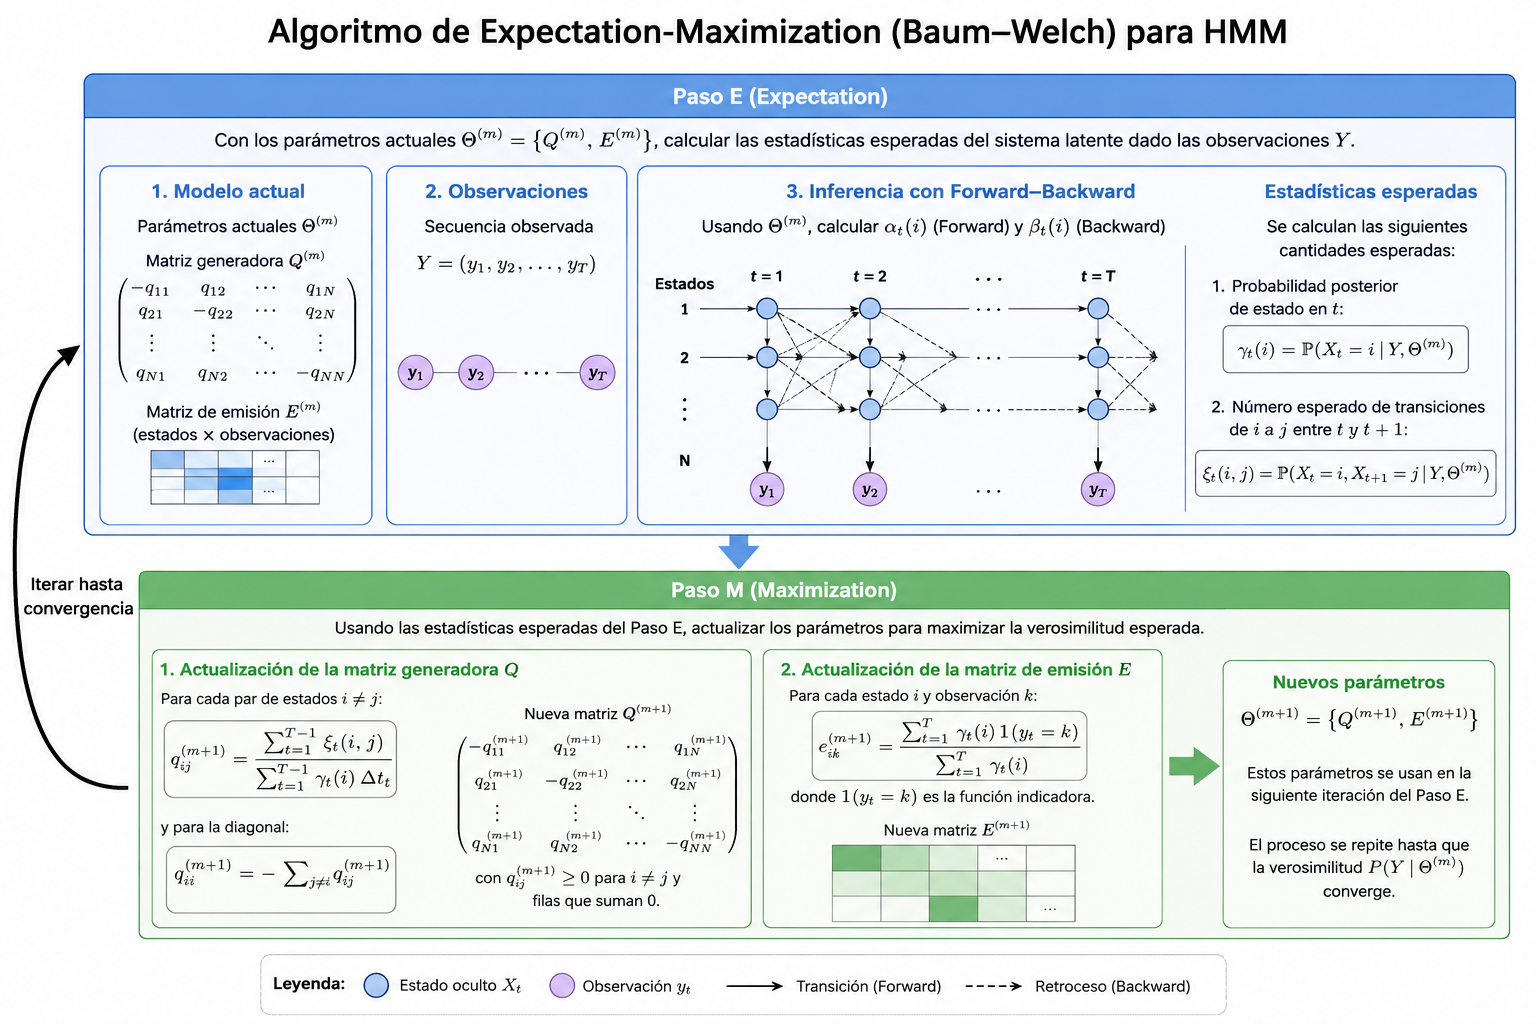
\includegraphics[width=8.33333in,height=\textheight,keepaspectratio]{imagenesHMM/ME_HMM.png}

}

\caption{\label{fig-ME}Esquema general del algoritmo
Expectation--Maximization (Baum--Welch) para un Modelo Oculto de Markov.
En el Paso E se estiman las probabilidades posteriores de los estados
ocultos y las transiciones esperadas mediante los algoritmos
Forward--Backward. En el Paso M se actualizan iterativamente la matriz
generadora y la matriz de emisión para maximizar la verosimilitud de las
observaciones.}

\end{figure}%

\phantomsection\label{refs}
\begin{CSLReferences}{1}{0}
\bibitem[\citeproctext]{ref-Norris1998}
Norris, J. R. 1998. \emph{Markov Chains}. Cambridge: Cambridge
University Press.

\bibitem[\citeproctext]{ref-Rudin1987}
Rudin, Walter. 1987. \emph{Real and Complex Analysis}. 3.ª ed. New York:
McGraw-Hill.

\end{CSLReferences}




\end{document}
